\subsection{Preventivo fase di Progettazione}

\subsubsection{Divisione oraria}
La seguente tabella rappresenta la distribuzione oraria dei ruoli per ogni componente del gruppo:
\rowcolors{2}{\evenRowColor}{\oddRowColor}
\renewcommand{\arraystretch}{2}
\begin{longtable}[h!] { C{3.5cm} C{1cm} C{1cm} C{1cm} C{1cm} C{1cm} C{1cm} C{2cm}}
\caption{Tabella della divisione oraria della Progettazione}\\
\rowcolor{\primaryColor}

\textcolor{\secondaryColor}{\textbf{Membro del gruppo}} & 
\textcolor{\secondaryColor}{\textbf{RE}} & 
\textcolor{\secondaryColor}{\textbf{AM}} & 
\textcolor{\secondaryColor}{\textbf{AN}} & 
\textcolor{\secondaryColor}{\textbf{PT}} & 
\textcolor{\secondaryColor}{\textbf{PR}} & 
\textcolor{\secondaryColor}{\textbf{VE}} & 
\textcolor{\secondaryColor}{\textbf{Ore complessive}}\\	
\endhead
        
\AW{}                     & 10  & - & - & 8 & 8 & 5 & 31 \\
\AT{}                     & -  & 10 & - & 7 & - & 14 & 31 \\
\AD{}                     & -  & 10 & - & 7 & 9 & 9 & 35 \\
\EC{}                     & 11  & - & 6 & - & 9 & 8 & 34 \\
\EM{}                     & -  & - & 7 & 7 & 11 & 9 & 34 \\
\FP{}                     & -  & - & 6 & 10 & 10 & 7 & 33 \\
\GG{}                     & -  & - & 5 & 10 & 11 & 7 & 33 \\
\textbf{Ore totali ruolo} & 21 & 20 & 24 & 49 & 58 & 59 & 231 \\

		
\end{longtable}
La suddivisione delle ore preventivate viene rappresentata anche sottoforma del seguente istogramma:\\
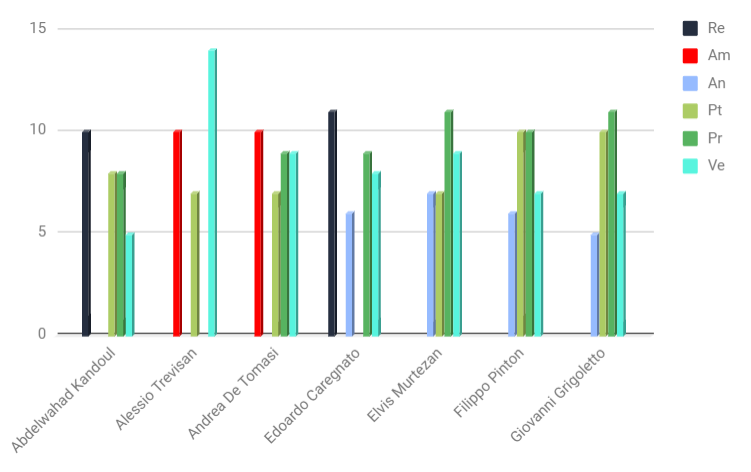
\includegraphics[width=1\textwidth]{./src/Preventivo/src/img/IstoProj.png}
%\begin{center}
%	\pgfplotsset{width=15.4cm, height=8.5cm}
%	\begin{tikzpicture}
%		\begin{axis}[
%			ybar stacked,
%			bar width=20pt,
%			legend style={
%				at={(0.5,-0.15)},
%				anchor=north,
%				legend columns=-1
%			},
%			symbolic x coords={Abdelwahad, Alessio, Andrea, Edoardo, Elvis, Filippo, Giovanni},
%			xtick=data
%		]
%			\legend{Responsabile, Amministratore, Analista, Progettista, Programmatore, Verificatore}
			% Responsabile
%			\addplot [ybar, fill=blue] coordinates {\ColonnaIstogramma{10}{0}{0}{11}{0}{0}{0}};
			% Amministratore
%			\addplot [ybar, fill=yellow] coordinates {\ColonnaIstogramma{0}{10}{10}{0}{0}{0}{0}};
			% Analista
%			\addplot [ybar, fill=red] coordinates {\ColonnaIstogramma{0}{0}{0}{6}{7}{6}{5}};
			% Progettista
%			\addplot [ybar, fill=green] coordinates {\ColonnaIstogramma{8}{7}{7}{0}{7}{10}{10}};
			% Programmatore
%			\addplot [ybar, fill=pink] coordinates {\ColonnaIstogramma{8}{0}{9}{9}{11}{10}{11}};
			% Verificatore
%			\addplot [ybar, fill=orange] coordinates {\ColonnaIstogramma{5}{14}{9}{8}{9}{7}{7}};
%		\end{axis}
%	\end{tikzpicture}
%\end{center}

\clearpage
\subsubsection{Costo risultante}
La seguente tabella rappresenta per ogni ruolo le ore totali preventivate ed il corrispondente costo in euro:
{
\rowcolors{2}{\evenRowColor}{\oddRowColor}
\renewcommand{\arraystretch}{2}
\begin{longtable}{ C{3cm} C{2cm} C{4cm}}
\caption{Tabella del costo risultante della Progettazione}\\
\rowcolor{\primaryColor}

\textcolor{\secondaryColor}{\textbf{Ruolo}} & 
\textcolor{\secondaryColor}{\textbf{Totale ore}} & 
\textcolor{\secondaryColor}{\textbf{Costo ruolo (in \euro{})}}\\	
\endhead
        
Responsabile    &  21 &  630 \\
Amministratore  &  20 &  400 \\
Analista        &  24 &  600 \\
Progettista     &  49 &  1078 \\
Programmatore   &  58 &  870 \\
Verificatore    &  59 &  885 \\
\textbf{Totale} &  231 & 4463 \\	
        	
\end{longtable}
}

\vskip 30pt %spazio verticale
La quantità di ore totali preventivate per ciascun ruolo viene rappresentata nel seguente areogramma:\\
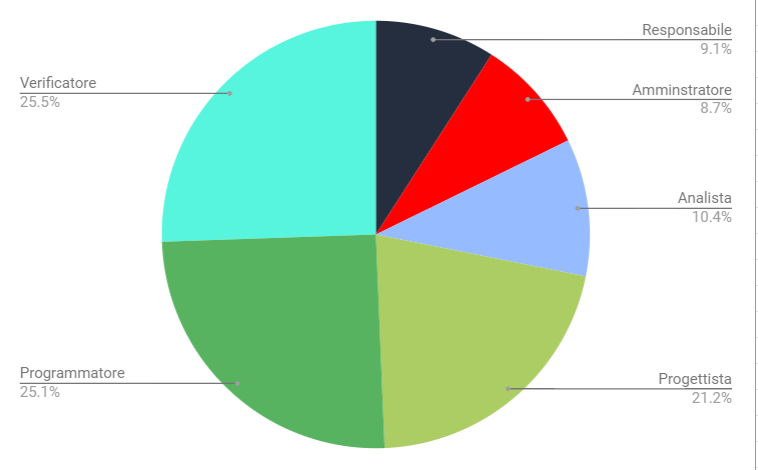
\includegraphics[width=1\textwidth]{./src/Preventivo/src/img/TortaProj.png}

%\begin{center}
%	\begin{tikzpicture}
%		\pie[rotate = 180, color={blue, yellow, red, green, pink, orange}] {
%			9/Responsabile,
%			9/Amministratore,
%			10/Analista,
%			21/Progettista,
%			25/Programmatore,
%			26/Verificatore
%		}
%	\end{tikzpicture}
%\end{center}